\subsection{Allgemeines}

\begin{itemize}
\item Linearer $(n,m)$-Code $C$
\item \textbf{\textit{a} x \textit{b} Generatormatrix:} $n = b$ und $m = a$
\item \textbf{\textit{a} x \textit{b} Kontrollmatrix:} $n = b$ und $m = a-b$
\end{itemize}

\subsection{Wichtige Formeln}

\begin{itemize}
\item \textbf{Blocklänge:} $\displaystyle n$
\item \textbf{Linear unabhängige Wörter/Dimension des Unterrraums $C$:} $m$
\item \textbf{Anzahl Codewörter:} $|C| = q^m$, wobei $q$ Anzahl Elemente in $C$
\item \textbf{Anzahl Wörter in Standardfeld:} $q^n$
\item \textbf{Anzahl Wörter/Zeilen in Syndromtabelle:} $q^{n-m}$
\item \textbf{Hamming Code:} $\displaystyle n = \frac{q^{n-m}-1}{q-1}$
\item \textbf{Schätzen der Codedistanz (Singleton-Schranke):} $d(C) \leq n - m + 1$ (obere Schranke)
\begin{itemize}
\item \textbf{Untere Schranke:} $d(C) \geq r + 1$, das bestimmte $r$ ist die untere schranke. Damit zeigt man auch, dass bei gegebener Kontrollmatrix $d(C)$ Wert $x$ hat.
\end{itemize}
\item \textbf{Fehlererkennend:} $(n - m)$
\item \textbf{Fehlerkorrigierend:} $\displaystyle \Bigl\lfloor \frac{(n - m)}{2} \Bigr\rfloor$
\item \textbf{t-fehlererkennend:} $d(C) \geq t + 1$, das ausgewählte $t$ ist, wie viel Fehler der Code erkennt
\item \textbf{t-fehlerkorrigierend:} $d(C) \geq 2t + 1$, das ausgewählte $t$ ist, wie viele Fehler der Code korrigiert
\item \textbf{t-ausfällekorrigierend:} $d(C) \geq t + 1$
\end{itemize}\

\newpage

\subsection{Allgemeines zu Matrizen}

\begin{minipage}{0.5\textwidth}
\textbf{Aufbau Generatormatrix:}

\begin{itemize}
\item $(m \times n)$ Generatormatrix
\item Beispiel: $m = 2, n = 5$
\begin{itemize}
\item[$\rightarrow$] $(2 \times 5)$ Generatormatrix
\end{itemize}
\end{itemize}\
\\

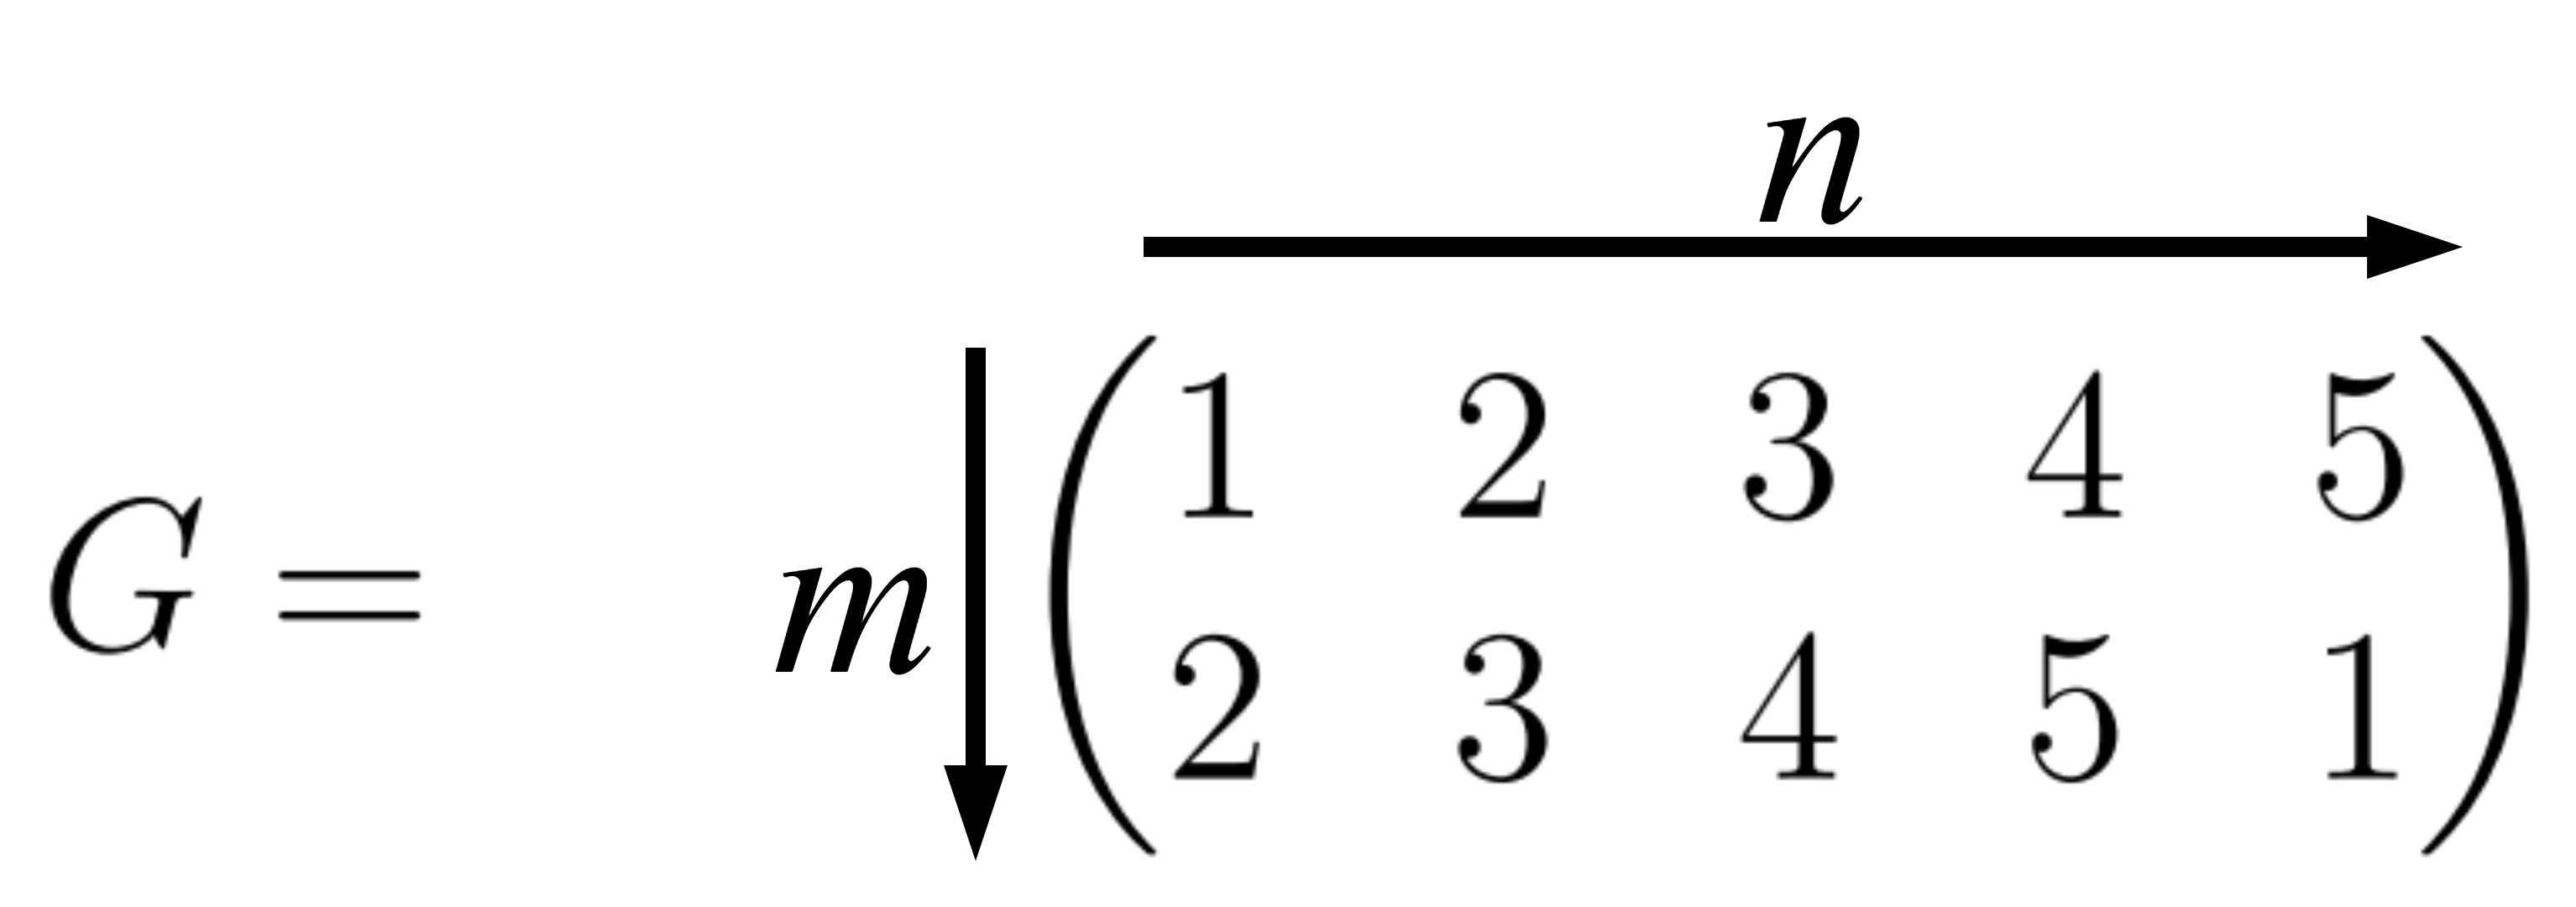
\includegraphics[width=0.6\textwidth]{graphics/generatormatrix.png}\\
\end{minipage}
\hfill
\begin{minipage}{0.5\textwidth}
\textbf{Aufbau Kontrollmatrix:}

\begin{itemize}
\item $(n \times n-m)$ Kontrollmatrix
\item Beispiel: $m= 2, n = 5$
\begin{itemize}
\item[$\rightarrow$] $(5 \times 5-2) = (5 \times 3)$ Kontrollmatrix
\end{itemize}
\end{itemize}\

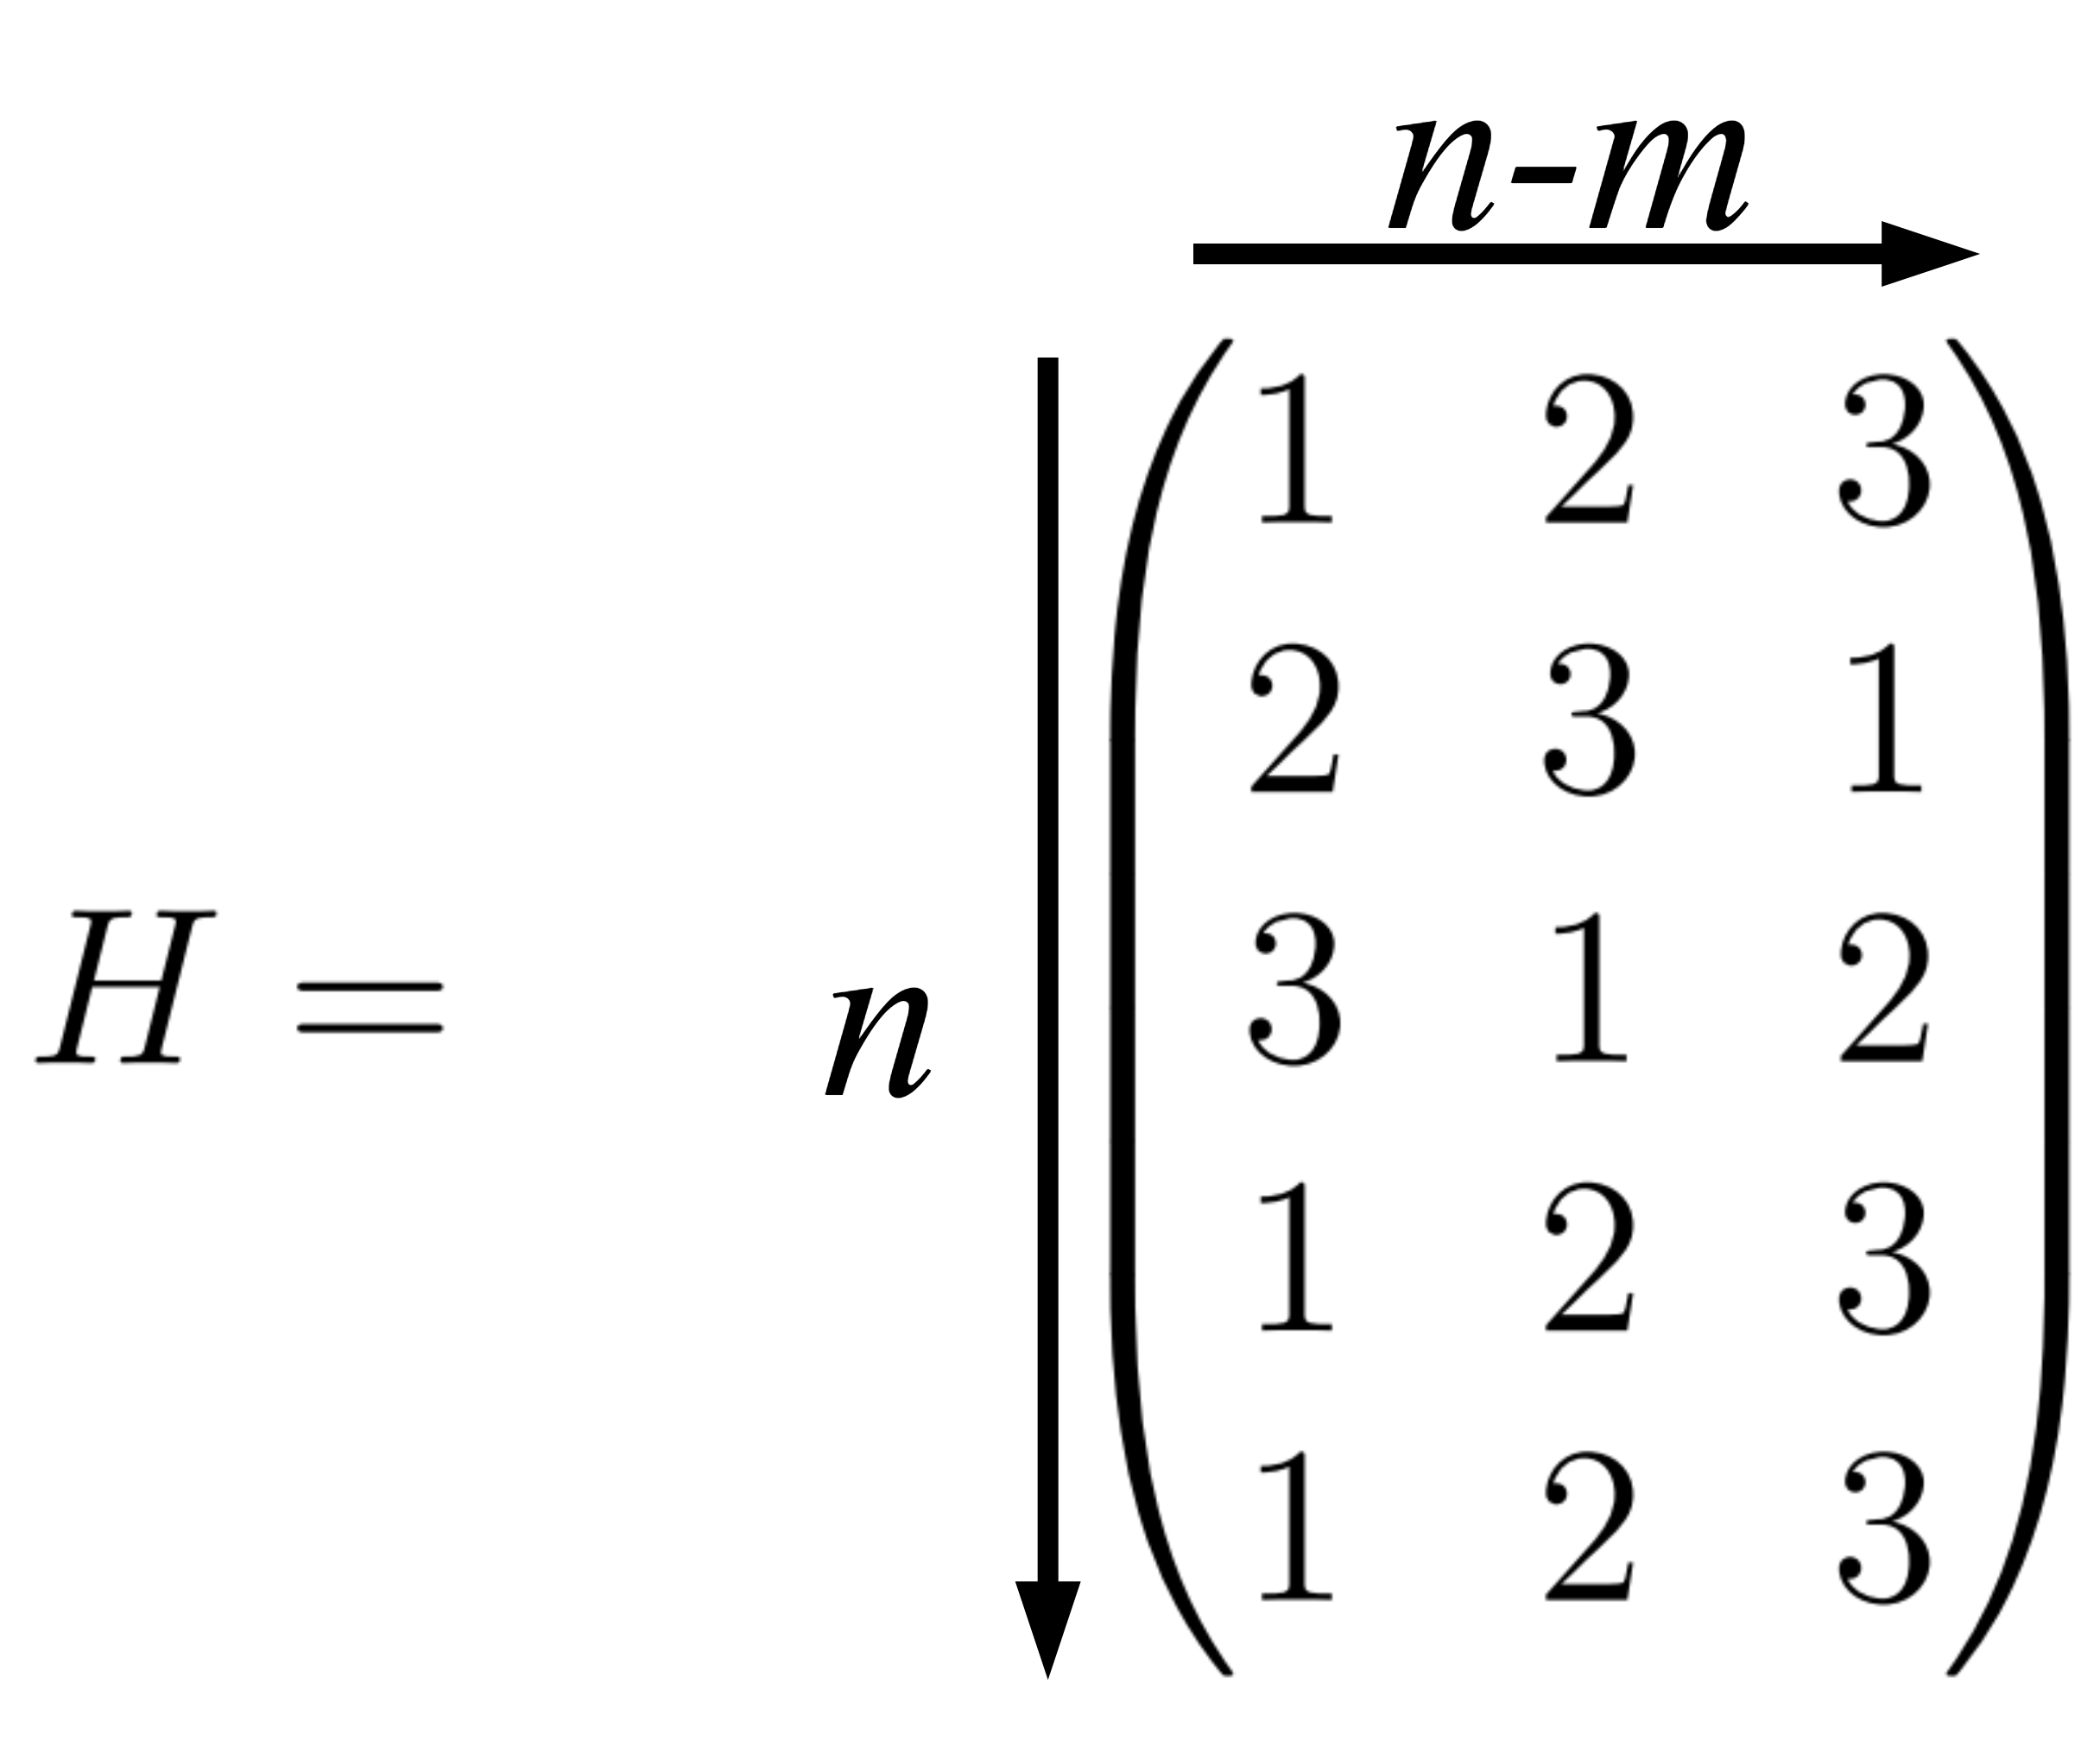
\includegraphics[width=0.5\textwidth]{graphics/kontrollmatrix.png}
\end{minipage}

\textbf{wort $\cdot$ matrix:}

$1010010 \cdot \begin{pmatrix}
1 & 1 & 1\\
1 & 0 & 1\\
0 & 1 & 1\\
1 & 1 & 0\\
1 & 0 & 0\\
0 & 1 & 0\\
0 & 0 & 1
\end{pmatrix} = \begin{pmatrix}
1\cdot1 & 1\cdot1 & 1\cdot1\\
1\cdot0 & 0\cdot0 & 1\cdot0\\
0\cdot1 & 1\cdot1 & 1\cdot1\\
1\cdot0 & 1\cdot0 & 0\cdot0\\
1\cdot0 & 0\cdot0 & 0\cdot0\\
0\cdot1 & 1\cdot1 & 0\cdot1\\
0\cdot0 & 0\cdot0 & 1\cdot0
\end{pmatrix} = \begin{pmatrix}
1 & 1 & 1\\
0 & 0 & 0\\
0 & 1 & 1\\
0 & 0 & 0\\
0 & 0 & 0\\
0 & 1 & 0\\
0 & 0 & 0
\end{pmatrix} = \begin{pmatrix}
\hspace{0.3cm}1 & | & \hspace{0.3cm}1 & | & \hspace{0.3cm}1\\
+0 & | & +0 & | & +0\\
+0 & | & +1 & | & +1\\
+0 & | & +0 & | & +0\\
+0 & | & +0 & | & +0\\
+0 & | & +1 & | & +0\\
+0 & \downarrow & +0 & \downarrow & +0
\end{pmatrix} = 110$\\~\\~\\

$1010010 \cdot \begin{pmatrix}
1 & 1 & 0 & 1 & 1 & 0 & 0\\
1 & 0 & 1 & 1 & 0 & 1 & 0\\
1 & 1 & 1 & 0 & 0 & 0 & 1
\end{pmatrix}^T = \begin{pmatrix}
1 \cdot 1 & 1 \cdot 0 & 0 \cdot 1 & 1 \cdot 0 & 1 \cdot 0 & 0 \cdot 1 & 0 \cdot 0\\
1 \cdot 1 & 0 \cdot 0 & 1 \cdot 1 & 1 \cdot 0 & 0 \cdot 0 & 1 \cdot 1 & 0 \cdot 0\\
1 \cdot 1 & 1 \cdot 0 & 1 \cdot 1 & 0 \cdot 0 & 0 \cdot 0 & 0 \cdot 1 & 1 \cdot 0
\end{pmatrix}^T =\\~\\~\\ \begin{pmatrix}
1 & 0 & 0 & 0 & 0 & 0 & 0\\
1 & 0 & 1 & 0 & 0 & 1 & 0\\
1 & 0 & 1 & 0 & 0 & 0 & 0
\end{pmatrix}^T = \begin{pmatrix}
1 & +0 & +0 & +0 & +0 & +0 & +0\\
- & - & - & - & - & - & \rightarrow\\
1 & +0 & +1 & +0 & +0 & +1 & +0\\
- & - & - & - & - & - & \rightarrow\\
1 & +0 & +1 & +0 & +0 & +0 & +0
\end{pmatrix}^T = 110$